% Copyright 2026 Sreeram Anil
% SPDX-License-Identifier: CC-BY-4.0
\chapter{State-of-health results over consecutive missions}
\label{ch:res-soh}

\section{The multi-flight study}

Capacity fade is invisible within one mission: a \SI{1}{\percent} loss of capacity changes the
terminal voltage of a discharge by less than the noise of the voltage sensor, and the
single-mission \code{aged\_cell} scenario of \cref{ch:res-cell_ecm} could only show which
estimators recover from a capacity that is \emph{already} \SI{15}{\percent} wrong. The
multi-flight benchmark (\code{bench\_soh}) asks the operational question instead. The cell
flies 120 consecutive eVTOL missions, one per day, each followed by a rest, a CC--CV recharge
at \SI{1}{C} to \SI{4.2}{\volt}, a second rest and a calendar-ageing storage interval; the plant
ages through the cycle and calendar laws of \cref{ch:ecm}, accelerated three-fold so that the
study spans a realistic end-of-life fade, from \SI{4.95}{} to \SI{3.95}{\ampere\hour}, in 120
days. The seven estimators that report a capacity run continuously through the whole study
without any reset, and their capacity estimate, averaged over the last tenth of each flight,
is compared with the true capacity at the end of that flight. The current sensor keeps its
nominal \SI{0.5}{\percent} scale-factor error throughout.

% Copyright 2026 Sreeram Anil
% SPDX-License-Identifier: CC-BY-4.0
\begin{table}[H]\centering\footnotesize\setlength{\tabcolsep}{3.5pt}\caption{Multi-flight state-of-health benchmark: 120 consecutive missions with accelerated ageing ($\times$3); capacity RMSE/MAE over flights 11--120, final capacity error, mean per-flight SOC RMSE and cost.}\label{tab:soh_overview}
\begin{tabular}{llrrrrr}\toprule estimator & family & RMSE $\hat Q$ [mAh] & MAE $\hat Q$ [mAh] & final [mAh] & SOC RMSE [\%] & ns/step \\ \midrule
DualEKF & soh & 26 & 25 & +29 & 0.42 & 1758 \\
JointEKF & soh & 26 & 25 & +21 & 0.11 & 1748 \\
JointUKF & soh & 29 & 28 & +22 & 0.10 & 3628 \\
DualUKF & soh & 33 & 32 & +22 & 0.14 & 2876 \\
AWTLS & soh & 49 & 41 & -35 & 0.84 & 986 \\
MMAE & adaptive\_kalman & 486 & 419 & +818 & 1.37 & 2277 \\
AdaptiveObserver & observers & 633 & 617 & +785 & 0.20 & 1390 \\
\bottomrule\end{tabular}\end{table}


\begin{figure}[H]\centering
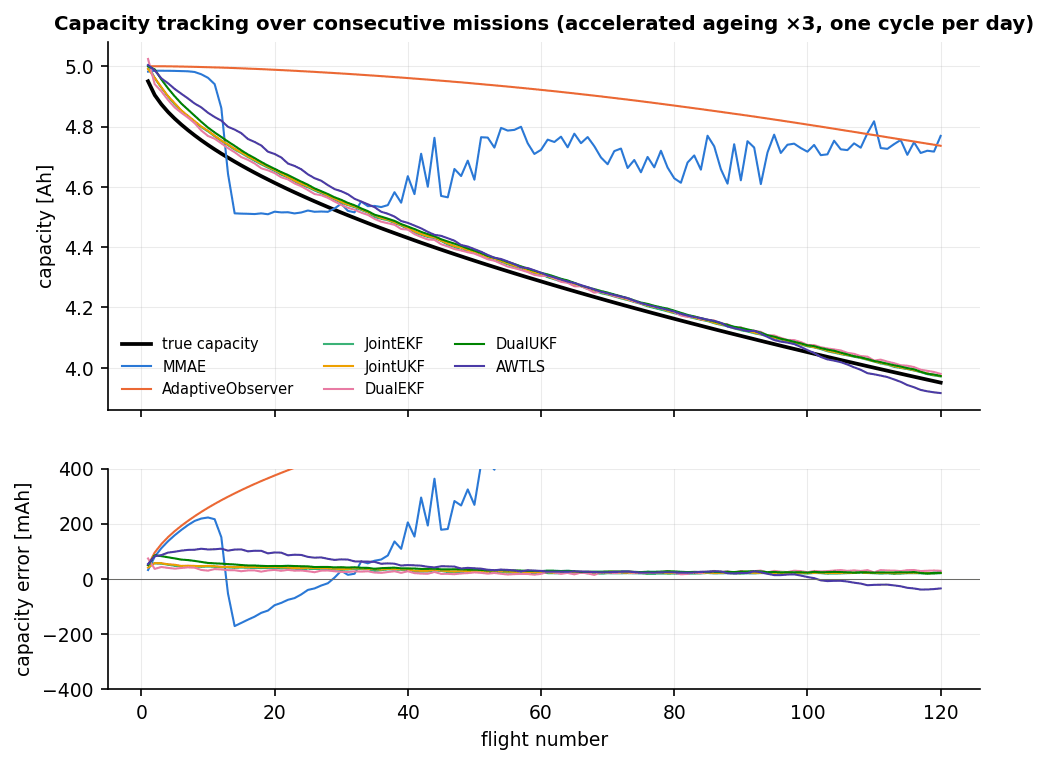
\includegraphics[width=\textwidth]{figures/soh_capacity_tracking.png}
\caption{Capacity tracking over 120 consecutive missions with three-fold accelerated ageing.
Top: estimated and true capacity; bottom: capacity error. The four joint and dual filters
track the fade to within \SIrange{25}{35}{\milli\ampere\hour}; the MMAE bank moves in steps
between its hypotheses; the adaptive observer's parameter loop is too slow to follow.}
\label{fig:res-soh}
\end{figure}

\section{What the numbers say}

\paragraph{The joint and dual filters track the fade to the sensor's accuracy.} Over flights
11--120 the dual EKF, joint EKF, joint UKF and dual UKF have capacity RMS errors of \num{26},
\num{26}, \num{29} and \SI{33}{\milli\ampere\hour}, i.e.\ \SIrange{0.5}{0.7}{\percent} of the
capacity, and their errors are almost entirely a constant positive offset of
\SIrange{+21}{+29}{\milli\ampere\hour} at the end of the study. That offset is the current
sensor: a scale factor of \num{1.005} makes every ampere-hour that passes the sensor
\SI{0.5}{\percent} larger than it is, so the capacity that explains the observed SOC swing is
\SI{0.5}{\percent} too large --- \SI{20}{\milli\ampere\hour} at \SI{4}{\ampere\hour}. The
filters are, in other words, reporting the capacity of the cell as seen through its current
sensor, exactly, and the residual after subtracting the sensor error is below
\SI{10}{\milli\ampere\hour}. Their transient is the prior: the \SIrange{40}{75}{\milli\ampere\hour} error of the
first flight decays over the first thirty to sixty flights to the sensor floor. There is no difference worth the name between the four in capacity accuracy; the two
EKF-based filters cost \SI{1.75}{\micro\second} per step, the two UKF-based ones \num{2.9} and
\SI{3.6}{\micro\second}, and the dual EKF has the smallest state (\SI{4.8}{\kilo\byte} against
\SI{8.8}{\kilo\byte} for the joint EKF, whose covariance is $6\times6$).

\paragraph{The per-flight SOC accuracy separates them.} The mean per-flight SOC RMSE over the
study is \SI{0.11}{\percent} for the joint EKF, \SI{0.10}{\percent} for the joint UKF,
\SI{0.14}{\percent} for the dual UKF and \SI{0.42}{\percent} for the dual EKF. The dual
structure pays for its smaller covariance with a slower SOC loop --- the state filter is told a
capacity that lags the parameter filter by design, and the cross-covariance between state and
parameter that the joint filter carries is exactly what is missing --- and the difference is
visible in every flight of the study. A BMS that needs both numbers at their best runs the
joint filter; the dual filter is the choice only where the $6\times6$ covariance does not fit
or where state and parameter must be updated at different rates.

\paragraph{AWTLS tracks with a lag and a sign change.} The approximate weighted total
least-squares capacity estimator, with its forgetting factor of \num{0.98}, reaches
\SI{49}{\milli\ampere\hour} RMS and ends \SI{35}{\milli\ampere\hour} \emph{low}. It fits a line
through accumulated charge against SOC change over a sliding window of flights, and a
monotone fade produces the classic lag of a windowed regression on a ramp; its estimate is
early in the study too high, as the others are, and crosses to the low side once the fade
rate has settled. Its per-flight SOC accuracy (\SI{0.84}{\percent}) is the worst of the five
because its inner EKF identifies only the capacity: the series resistance, which the plant
raises by \num{2.5} times the capacity-loss fraction as the cell ages, stays at its
beginning-of-life value, and the growing overpotential error is absorbed by the SOC. The joint
and dual filters carry $R_0$ as a second parameter and do not have this problem.

\paragraph{The hypothesis bank and the adaptive observer do not track.} The MMAE bank runs
three filters at fixed capacity hypotheses and reports the weighted mean; it can only follow
the fade in steps between hypotheses, and its trace in \cref{fig:res-soh} does exactly that,
holding \SI{4.51}{\ampere\hour} from flight 15 to flight 30 and then wandering between
\SI{4.6}{} and \SI{4.8}{\ampere\hour} as the likelihoods of the two remaining hypotheses trade
off; the RMS error is \SI{486}{\milli\ampere\hour}. The adaptive observer's capacity output
moves in the right direction but ten times too slowly (\SI{4.73}{\ampere\hour} at the end,
\SI{633}{\milli\ampere\hour} RMS): its parameter-adaptation gain is set for stability of the
certified state loop, and \cref{ch:adaptiveobserver} is explicit that the output should be read
as a trend indicator and not as a capacity. The adaptive observer keeps its SOC accuracy (\SI{0.20}{\percent} per flight) despite the
wrong capacity, because its certified state loop corrects from the voltage --- the same
observation as in \cref{ch:res-cell_ecm}, that a state estimator with a voltage correction
survives a capacity error it cannot identify; the MMAE bank does not (\SI{1.37}{\percent}),
because its SOC is a mixture of filters whose capacities are far from the truth.

\section{What the state-of-health results say}

Capacity is identifiable over consecutive missions to the accuracy of the current sensor's
scale factor, by any of the joint or dual filters, without excitation beyond what the missions
themselves provide, and without resets. The residual error is a sensor calibration problem: a
\SI{0.5}{\percent} scale-factor error is a \SI{0.5}{\percent} capacity error, permanently, and
no estimator can separate the two from voltage and current alone. The joint EKF is the
recommendation; the dual EKF matches its capacity accuracy at the same cost but with four times
the SOC error, and is worth choosing only for its smaller state or a decoupled update rate. A capacity estimate from a method that was not designed to identify capacity --- a
hypothesis bank with coarse steps, or the adaptation loop of a state observer --- should be
displayed as a health trend, not used as the capacity in the SOC computation.
